% XCircuit output "scanChain.tex" for LaTeX input from scanChain.ps
\def\putbox#1#2#3#4{\makebox[0in][l]{\makebox[#1][l]{}\raisebox{\baselineskip}[0in][0in]{\raisebox{#2}[0in][0in]{\scalebox{#3}{#4}}}}}
\def\rightbox#1{\makebox[0in][r]{#1}}
\def\centbox#1{\makebox[0in]{#1}}
\def\topbox#1{\raisebox{-0.60\baselineskip}[0in][0in]{#1}}
\def\midbox#1{\raisebox{-0.20\baselineskip}[0in][0in]{#1}}
   \scalebox{1}{
   \normalsize
   \parbox{7.5in}{
   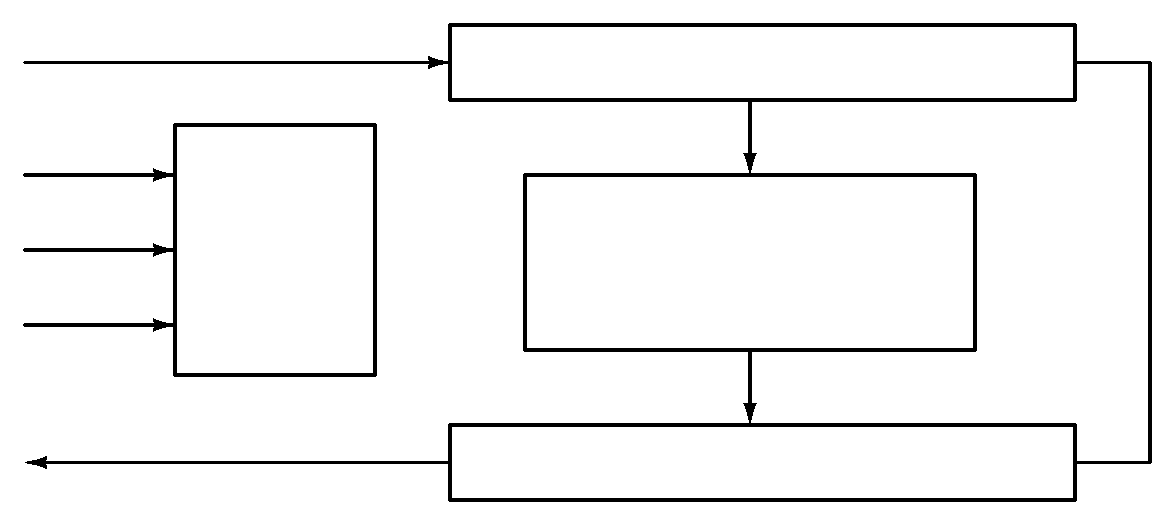
\includegraphics[scale=0.75]{scanChain.eps}\\
   % translate x=960 y=320 scale 0.38
   \putbox{3.44in}{1.16in}{1.20}{DUT}%
   \putbox{3.29in}{2.15in}{1.20}{In Register}%
   \putbox{3.29in}{0.15in}{1.20}{Out Register}%
   \putbox{1.1in}{1.41in}{1.20}{TAP}%
   \putbox{0.9in}{1.15in}{1.20}{Controller}%
   \putbox{3.77in}{1.82in}{1.20}{dut\_in}%
   \putbox{3.77in}{0.55in}{1.20}{dut\_out}%
   \putbox{0.1in}{1.78in}{1.20}{TMS}%
   \putbox{0.1in}{1.38in}{1.20}{TCLK}%
   \putbox{0.1in}{0.98in}{1.20}{TRST}%
   \putbox{0.1in}{2.28in}{1.20}{TDI}%\\
   \putbox{0.1in}{0.32in}{1.20}{TDO}%
   } % close 'parbox'
   } % close 'scalebox'
   \vspace{-\baselineskip} % this is not necessary, but looks better
